\documentclass[border=5pt]{standalone}
\usepackage{pgfplots}
\pgfplotsset{compat=1.18}
\usepackage{siunitx}
\usepackage{tikz}
\usetikzlibrary{calc}

\definecolor{lr1}{RGB}{31,119,180}
\definecolor{lr2}{RGB}{255,127,14}
\definecolor{lr3}{RGB}{143,0,255}
\definecolor{lr4}{RGB}{44,160,44}

\begin{document}
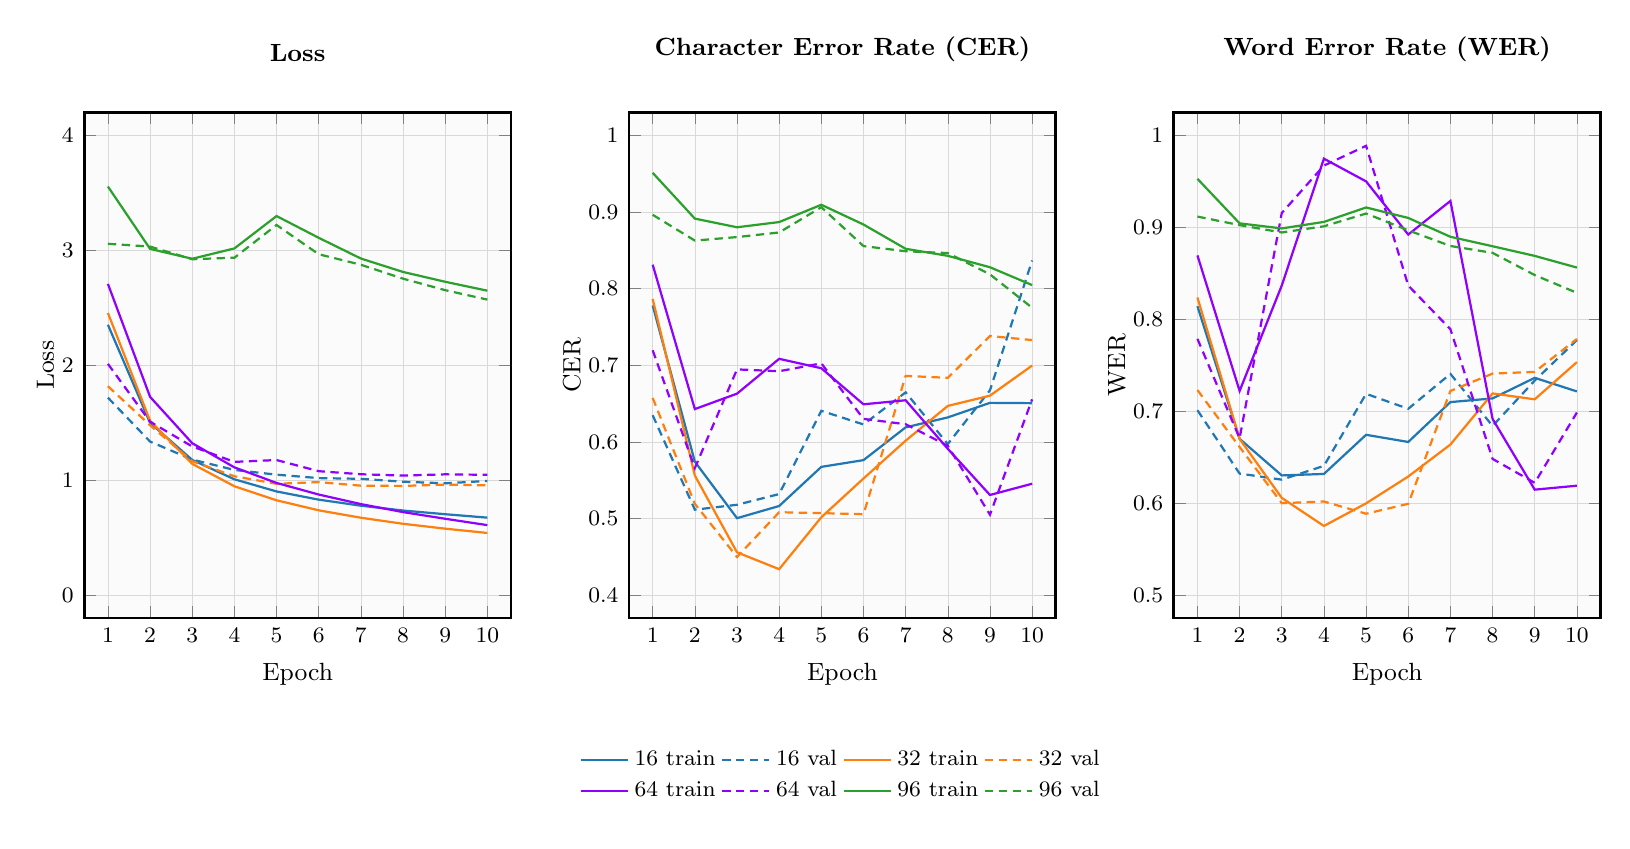
\begin{tikzpicture}[remember picture]

    % Графік 1: Loss
    \begin{axis}[
        name=plot1,
        width=7cm,
        height=8cm,
        xlabel={Epoch},
        ylabel={Loss},
        ylabel style={yshift=-0.15cm},
        xmin=0.9, xmax=10.1,
        ymin=0, ymax=4,
        xtick={1,2,3,4,5,6,7,8,9,10},
        grid=both,
        grid style={line width=.1pt, draw=gray!10},
        major grid style={line width=.2pt,draw=gray!30},
        title={Loss},
        axis background/.style={fill=gray!3},
        title style={yshift=3mm, font=\small\bfseries},
        label style={font=\small},
        tick label style={font=\footnotesize},
        line width=1pt,
        enlarge x limits=0.05,
        enlarge y limits=0.05,
        every axis plot/.append style={mark size=2pt},
        legend to name=commonlegend,
        legend columns=4,
        legend style={draw=none, fill=none, font=\footnotesize}
    ]
        % 16
        \addplot[color=lr1, thick] coordinates {
            (1,2.3535) (2,1.4991) (3,1.1764) (4,1.0078) (5,0.9020) 
            (6,0.8306) (7,0.7780) (8,0.7358) (9,0.7038) (10,0.6739)};
        \addplot[color=lr1, thick, densely dashed] coordinates {
            (1,1.7187) (2,1.3363) (3,1.1796) (4,1.0892) (5,1.0481) 
            (6,1.0182) (7,1.0121) (8,0.9868) (9,0.9728) (10,0.9936)};

        % 32
        \addplot[color=lr2, thick] coordinates {
            (1,2.4561) (2,1.5176) (3,1.1423) (4,0.9474) (5,0.8250) 
            (6,0.7377) (7,0.6732) (8,0.6205) (9,0.5780) (10,0.5406)};
        \addplot[color=lr2,  thick, densely dashed] coordinates {
            (1,1.8180) (2,1.4784) (3,1.1651) (4,1.0345) (5,0.9685) 
            (6,0.9834) (7,0.9522) (8,0.9503) (9,0.9616) (10,0.9550)};

        % 64
        \addplot[color=lr3,  thick] coordinates {
            (1,2.7090) (2,1.7256) (3,1.3219) (4,1.1118) (5,0.9761) 
            (6,0.8751) (7,0.7920) (8,0.7222) (9,0.6642) (10,0.6087)};
        \addplot[color=lr3,  thick, densely dashed] coordinates {
            (1,2.0126) (2,1.5092) (3,1.2936) (4,1.1594) (5,1.1754) 
            (6,1.0785) (7,1.0518) (8,1.0400) (9,1.0511) (10,1.0468)};

        % 96
        \addplot[color=lr4,  thick] coordinates {
            (1,3.5568) (2,3.0138) (3,2.9279) (4,3.0178) (5,3.2997) 
            (6,3.1104) (7,2.9299) (8,2.8130) (9,2.7275) (10,2.6498)};
        \addplot[color=lr4,  thick, densely dashed] coordinates {
            (1,3.0581) (2,3.0341) (3,2.9237) (4,2.9370) (5,3.2217) 
            (6,2.9673) (7,2.8758) (8,2.7545) (9,2.6544) (10,2.5723)};

        \legend{16 train, 16 val, 32 train, 32 val, 64 train, 64 val, 96 train, 96 val}
    \end{axis}

    % Графік 2: CER, розташовується праворуч від plot1
    \begin{axis}[
        name=plot2,
        at={($(plot1.east)+(1.5cm,0)$)},
        anchor=west,
        width=7cm,
        height=8cm,
        xlabel={Epoch},
        ylabel={CER},
        ylabel style={yshift=-0.15cm},
        xmin=0.9, xmax=10.1,
        ymin=0.4, ymax=1.0,
        xtick={1,2,3,4,5,6,7,8,9,10},
        grid=both,
        grid style={line width=.1pt, draw=gray!10},
        major grid style={line width=.2pt,draw=gray!30},
        title={Character Error Rate (CER)},
        axis background/.style={fill=gray!3},
        title style={yshift=3mm, font=\small\bfseries},
        label style={font=\small},
        tick label style={font=\footnotesize},
        line width=1pt,
        enlarge x limits=0.05,
        enlarge y limits=0.05,
        every axis plot/.append style={mark size=2pt}
    ]
        % 16
        \addplot[color=lr1, , thick] coordinates {
            (1,0.7782) (2,0.5742) (3,0.5004) (4,0.5163) (5,0.5674) 
            (6,0.5762) (7,0.6190) (8,0.6320) (9,0.6510) (10,0.6506)};
        \addplot[color=lr1, , thick, densely dashed] coordinates {
            (1,0.6348) (2,0.5115) (3,0.5179) (4,0.5319) (5,0.6406) 
            (6,0.6228) (7,0.6647) (8,0.5972) (9,0.6674) (10,0.8369)};

        % 32
        \addplot[color=lr2,  thick] coordinates {
            (1,0.7867) (2,0.5561) (3,0.4558) (4,0.4338) (5,0.5016) 
            (6,0.5522) (7,0.6016) (8,0.6470) (9,0.6604) (10,0.6997)};
        \addplot[color=lr2,  thick, densely dashed] coordinates {
            (1,0.6574) (2,0.5192) (3,0.4497) (4,0.5082) (5,0.5070) 
            (6,0.5056) (7,0.6862) (8,0.6837) (9,0.7383) (10,0.7330)};

        % 64
        \addplot[color=lr3,  thick] coordinates {
            (1,0.8314) (2,0.6429) (3,0.6630) (4,0.7085) (5,0.6962) 
            (6,0.6491) (7,0.6544) (8,0.5910) (9,0.5307) (10,0.5454)};
        \addplot[color=lr3,  thick, densely dashed] coordinates {
            (1,0.7196) (2,0.5659) (3,0.6947) (4,0.6923) (5,0.7026) 
            (6,0.6301) (7,0.6231) (8,0.5949) (9,0.5050) (10,0.6556)};

        % 96
        \addplot[color=lr4,  thick] coordinates {
            (1,0.9514) (2,0.8916) (3,0.8803) (4,0.8871) (5,0.9097) 
            (6,0.8839) (7,0.8522) (8,0.8430) (9,0.8281) (10,0.8048)};
        \addplot[color=lr4,  thick, densely dashed] coordinates {
            (1,0.8966) (2,0.8629) (3,0.8675) (4,0.8735) (5,0.9065) 
            (6,0.8557) (7,0.8490) (8,0.8466) (9,0.8188) (10,0.7752)};
    \end{axis}

    % Графік 3: WER, розташовується праворуч від plot2
    \begin{axis}[
        name=plot3,
        at={($(plot2.east)+(1.5cm,0)$)},
        anchor=west,
        width=7cm,
        height=8cm,
        xlabel={Epoch},
        ylabel={WER},
        ylabel style={yshift=-0.15cm},
        xmin=0.9, xmax=10.1,
        ymin=0.5, ymax=1.0,
        xtick={1,2,3,4,5,6,7,8,9,10},
        grid=both,
        grid style={line width=.1pt, draw=gray!10},
        major grid style={line width=.2pt,draw=gray!30},
        title={Word Error Rate (WER)},
        axis background/.style={fill=gray!3},
        title style={yshift=3mm, font=\small\bfseries},
        label style={font=\small},
        tick label style={font=\footnotesize},
        line width=1pt,
        enlarge x limits=0.05,
        enlarge y limits=0.05,
        every axis plot/.append style={mark size=2pt}
    ]
        % 16
        \addplot[color=lr1, , thick] coordinates {
            (1,0.8143) (2,0.6700) (3,0.6302) (4,0.6318) (5,0.6744) 
            (6,0.6666) (7,0.7100) (8,0.7140) (9,0.7364) (10,0.7216)};
        \addplot[color=lr1, , thick, densely dashed] coordinates {
            (1,0.7012) (2,0.6322) (3,0.6256) (4,0.6406) (5,0.7190) 
            (6,0.7027) (7,0.7407) (8,0.6840) (9,0.7334) (10,0.7775)};

        % 32
        \addplot[color=lr2,  thick] coordinates {
            (1,0.8238) (2,0.6699) (3,0.6057) (4,0.5752) (5,0.5998) 
            (6,0.6290) (7,0.6638) (8,0.7194) (9,0.7130) (10,0.7535)};
        \addplot[color=lr2,  thick, densely dashed] coordinates {
            (1,0.7231) (2,0.6611) (3,0.6000) (4,0.6018) (5,0.5885) 
            (6,0.5993) (7,0.7221) (8,0.7410) (9,0.7429) (10,0.7787)};

        % 64
        \addplot[color=lr3,  thick] coordinates {
            (1,0.8696) (2,0.7222) (3,0.8369) (4,0.9749) (5,0.9502) 
            (6,0.8923) (7,0.9289) (8,0.6917) (9,0.6147) (10,0.6190)};
        \addplot[color=lr3,  thick, densely dashed] coordinates {
            (1,0.7788) (2,0.6706) (3,0.9158) (4,0.9674) (5,0.9889) 
            (6,0.8368) (7,0.7893) (8,0.6482) (9,0.6221) (10,0.6986)};

        % 96
        \addplot[color=lr4,  thick] coordinates {
            (1,0.9530) (2,0.9045) (3,0.8990) (4,0.9061) (5,0.9218) 
            (6,0.9104) (7,0.8899) (8,0.8796) (9,0.8691) (10,0.8564)};
        \addplot[color=lr4,  thick, densely dashed] coordinates {
            (1,0.9119) (2,0.9026) (3,0.8946) (4,0.9013) (5,0.9152) 
            (6,0.8969) (7,0.8799) (8,0.8724) (9,0.8482) (10,0.8289)};
    \end{axis}

    % Розміщення загальної легенди під усіма графіками
    \node at ($(plot1.south)!0.5!(plot3.south)+(0,-2.0cm)$) {\pgfplotslegendfromname{commonlegend}};
    
\end{tikzpicture}
\end{document}